\iffalse
\documentclass[12pt]{article}
\usepackage{graphicx}
\usepackage[none]{hyphenat}
\usepackage{graphicx}
\usepackage{listings}
\usepackage[english]{babel}
\usepackage{graphicx}
\usepackage{caption} 
\usepackage{hyperref}
\usepackage{booktabs}
\usepackage{array}
\usepackage{amsmath}   % for having text in math mode
\usepackage{extarrows} % for Row operations arrows
\usepackage{listings}
\lstset{
  frame=single,
  breaklines=true
}
  
%Following 2 lines were added to remove the blank page at the beginning
\usepackage{atbegshi}% http://ctan.org/pkg/atbegshi
\AtBeginDocument{\AtBeginShipoutNext{\AtBeginShipoutDiscard}}


%New macro definitions
\newcommand{\mydet}[1]{\ensuremath{\begin{vmatrix}#1\end{vmatrix}}}
\providecommand{\brak}[1]{\ensuremath{\left(#1\right)}}
\providecommand{\norm}[1]{\left\lVert#1\right\rVert}
\newcommand{\solution}{\noindent \textbf{Solution: }}
\newcommand{\myvec}[1]{\ensuremath{\begin{pmatrix}#1\end{pmatrix}}}
\let\vec\mathbf

\begin{document}

\begin{center}
\title{\textbf{Equation  of Line}}
\date{\vspace{-5ex}} %Not to print date automatically
\maketitle
\end{center}
\setcounter{page}{1}

\section{11$^{th}$ Maths - Chapter 10}
This is Problem-12 from Exercise 10.2
\begin{enumerate}
		\fi
\item Find the equation of a line that cuts off equal intercepts on the coordinate axes and passes through the point $(2,3)$.  
	\\
\solution 
Let $\vec{P}(a,0), \text{ and } \vec{Q}(0,a)$ be the 2 points on x and y-axes respectively having $a$ as the intercept on both the axes. We know that the the direction vector $\vec{m}$ of the line joining two points $\vec{P}, \vec{Q}$ is given by  
\begin{align}
\vec{m} &=   \vec{P} - \vec{Q} \\
        &=   \myvec{
		a \\
		0 
		} - \myvec{
		   0 \\
		   a
		}  = a\myvec{ 
                     1 \\
		   -1 
        		}  \equiv \myvec{
                           1 \\
			   -1 
		         } 
\end{align}
Thus, the normal vector $\vec{n}$ to the line is given as
\begin{align}
\vec{n} &=  \myvec{
		     1 \\
		     1
	     } 
\end{align}
The equation of a line with normal vector $\vec{n}$ and passing through a point $\vec{A}(2,3)$ is given by
\begin{align}
	\vec{n}^\top\brak{\vec{x}-\vec{A}} &= 0 \\
	\myvec { 1 & 1 } \brak{ \vec{ x  - \myvec{ 2 \\
                                   3
			     }
		}}  &= 0  \\
	\myvec{ 1 & 1} \vec{x} -5 &= 0 \\
        \label{eq:11/10/2/12/1}
	\myvec{ 1 & 1} \vec{x}  &= 5 
\end{align}
To find the intercepts, we know that, since $\vec{P} \text{ and } \vec{Q}$ lie on the straight line, they should satisfy \eqref{eq:11/10/2/12/1}.
\begin{align}
	\myvec{ 1 & 1} \vec{P}  &= 5 \\
	\myvec{ 1 & 1} \myvec{a \\
	                      0 }  &= 5 \\ 
	a + 0 &= 5 \\
	a &= 5 
\end{align}
Both $\vec{P} \text{ and } \vec{Q}$ have the same intercept value, hence the intercept on both x and y-axes is 5 units. The line segment is as shown in Fig. \ref{fig:11/10/2/12/Fig1}.
\begin{figure}[!h]
	\begin{center}
		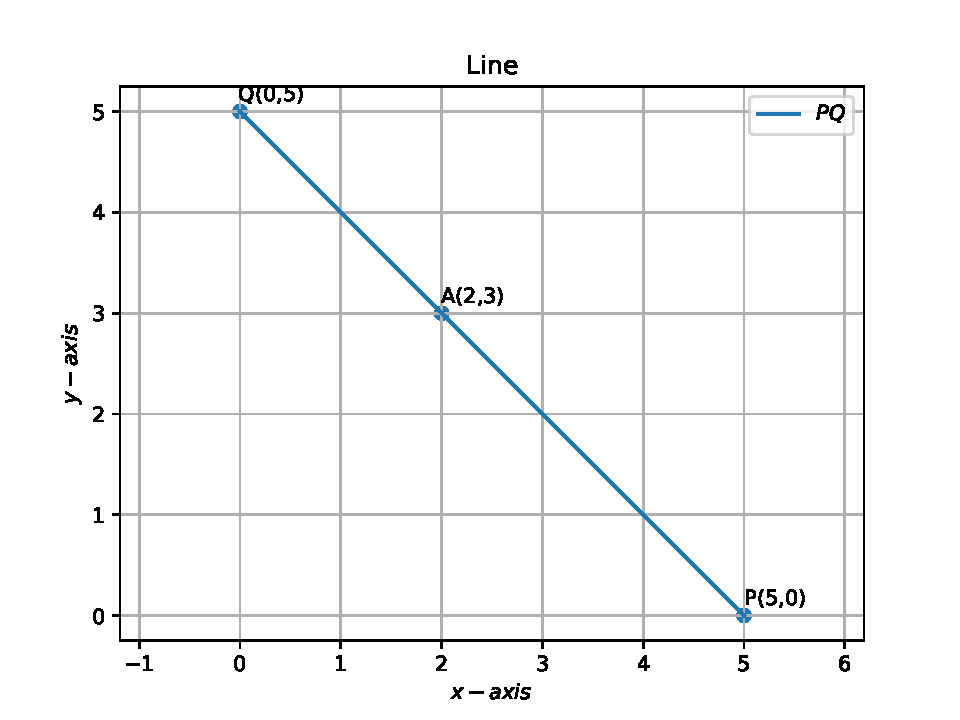
\includegraphics[width=\columnwidth]{chapters/11/10/2/12/figs/problem12.pdf}
	\end{center}
\caption{}
\label{fig:11/10/2/12/Fig1}
\end{figure}

